\chapter{Activity-Lifecycle unter Android}
\begin{figure}[h]
  \centering
  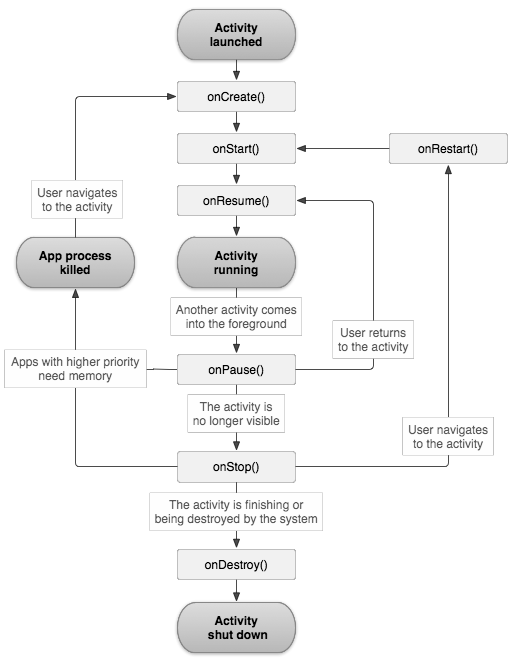
\includegraphics[keepaspectratio, height=0.6\textheight]{concept/lifecycle}
  \src{https://developer.android.com/guide/components/activities/activity-lifecycle.html}{07.03.2018}
  \caption{\emph{Activity Lifecycle}}
  \label{fig:lifecycle}
\end{figure}

\chapter{UML-Diagramm des ersten Prototyps}\label{chap:uml}
\begin{figure}[h]
  \centering
  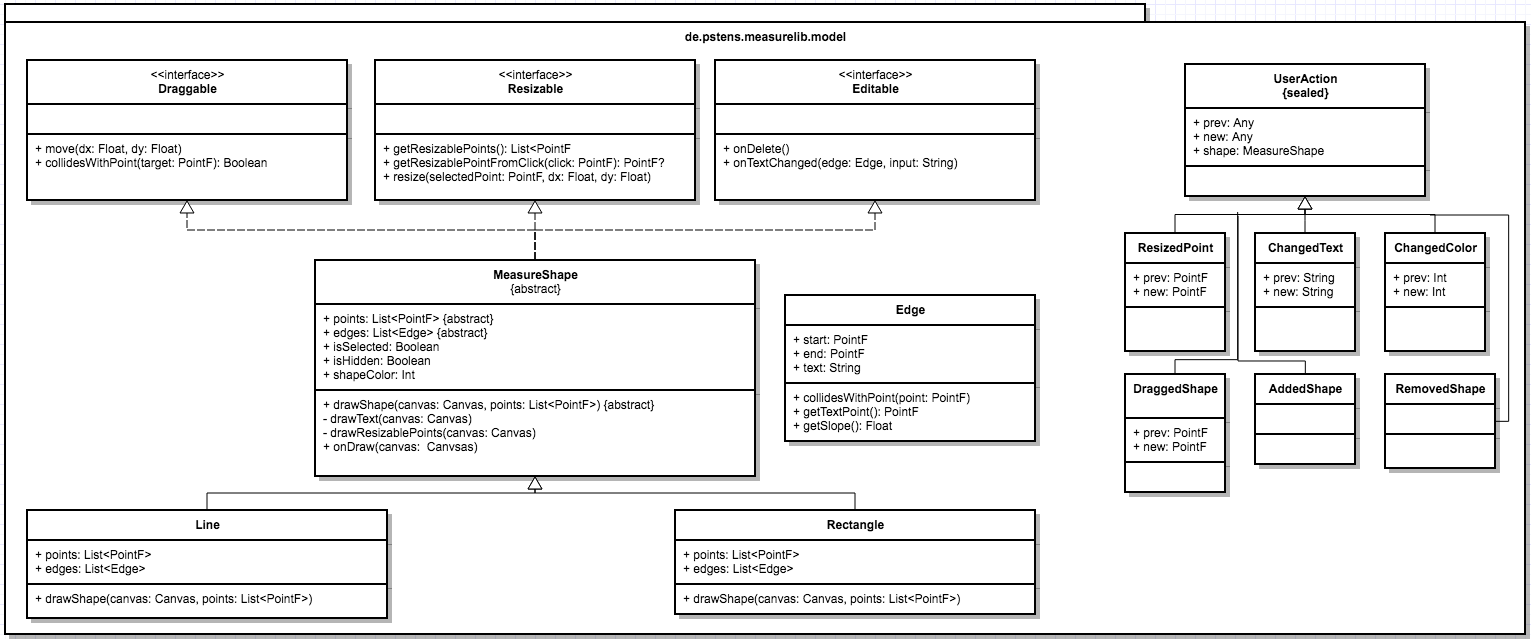
\includegraphics[keepaspectratio, width=\textwidth]{prototype1/model}
  \caption{Datenmodell (Model)}
  \label{fig:model}
\end{figure}

\begin{figure}[h]
  \centering
  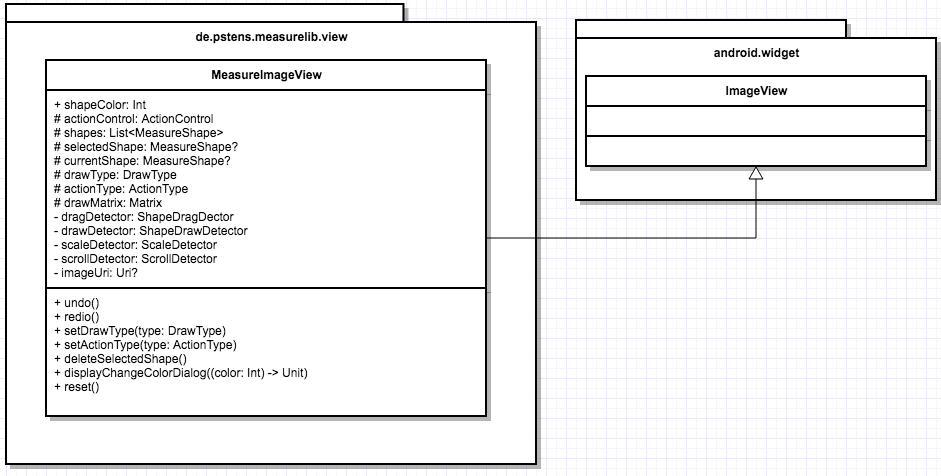
\includegraphics[keepaspectratio, width=\textwidth]{prototype1/view}
  \caption{Präsentationskomponente (View)}
  \label{fig:view}
\end{figure}

\begin{figure}[h]
  \centering
  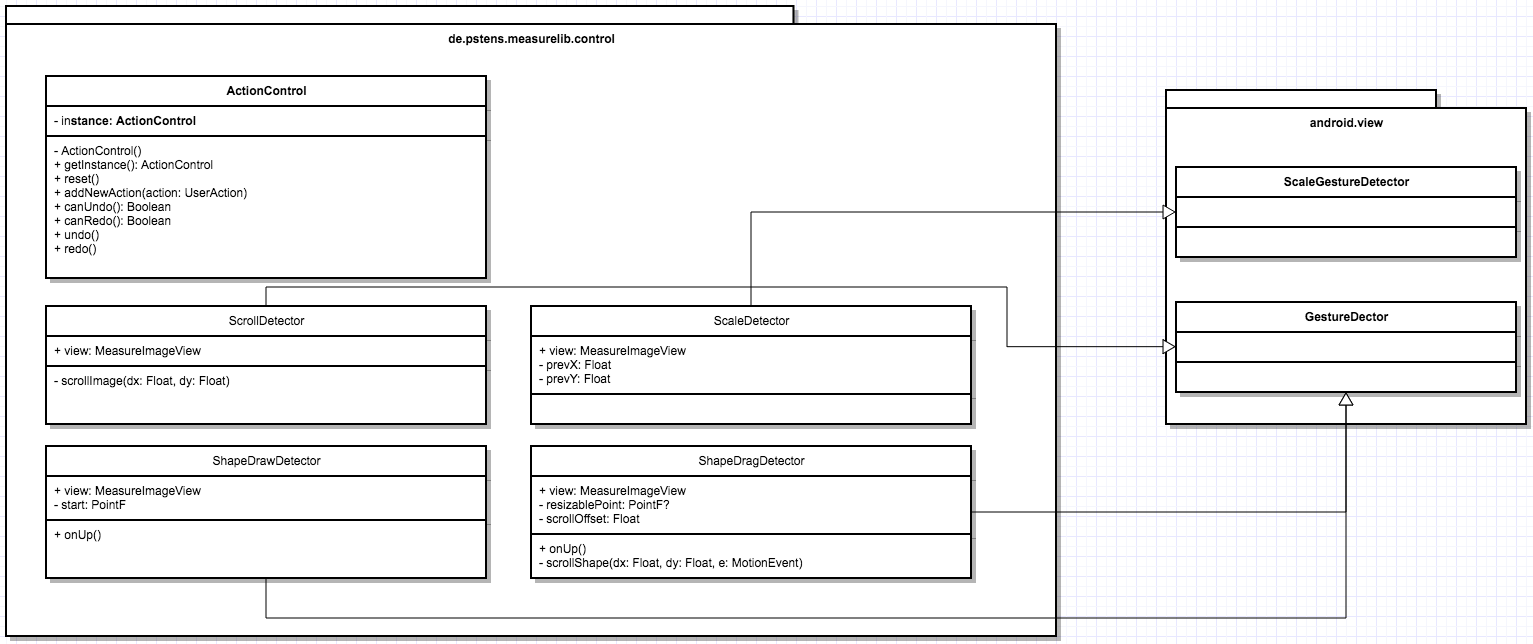
\includegraphics[keepaspectratio, width=\textwidth]{prototype1/control}
  \caption{Programmsteuerung (Control)}
  \label{fig:control}
\end{figure}

\chapter{Verbreitung der verschiedenen Android-Versionen Dezember 2017}
\begin{figure}[h]
  \centering
  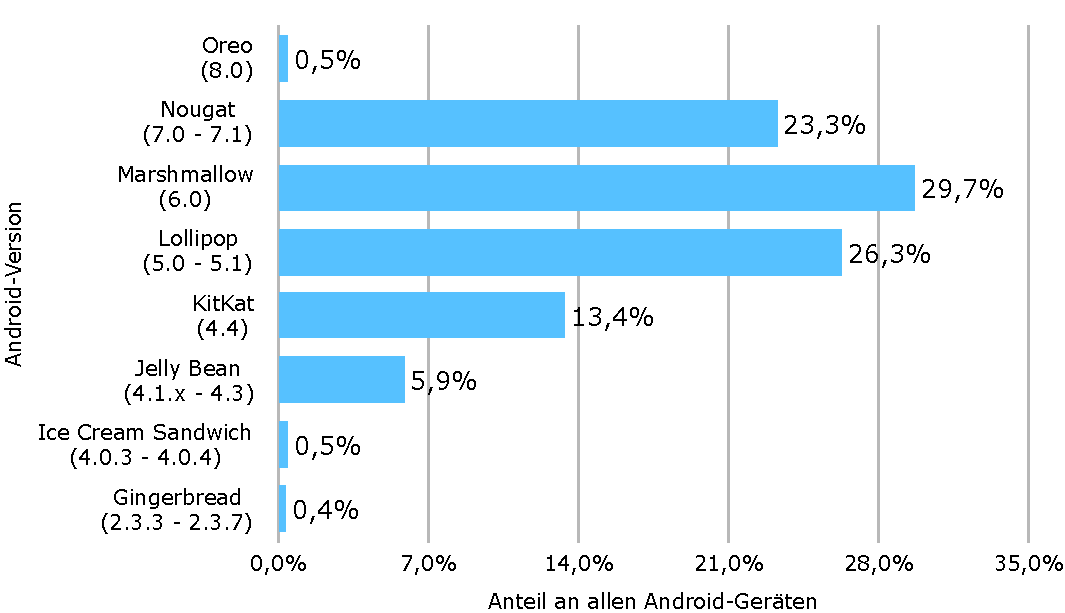
\includegraphics[keepaspectratio, width=\textwidth]{prototype2/androidchart}
  \par\raggedleft\footnotesize In Anlehnung an: \url{https://developer.android.com/about/dashboards/index.html} (Abruf:~02.01.2018)
  \caption{Anteil der verschiedenen Android-Versionen an allen Geräten mit Android OS weltweit im Zeitraum vom 5. bis 11. Dezember 2017}
  \label{fig:versionchart}
\end{figure}

\chapter{Anzahl hochgeladener Bilder am Standort Paderborn und Stara Zagora}
\begin{figure}[h]
  \centering
  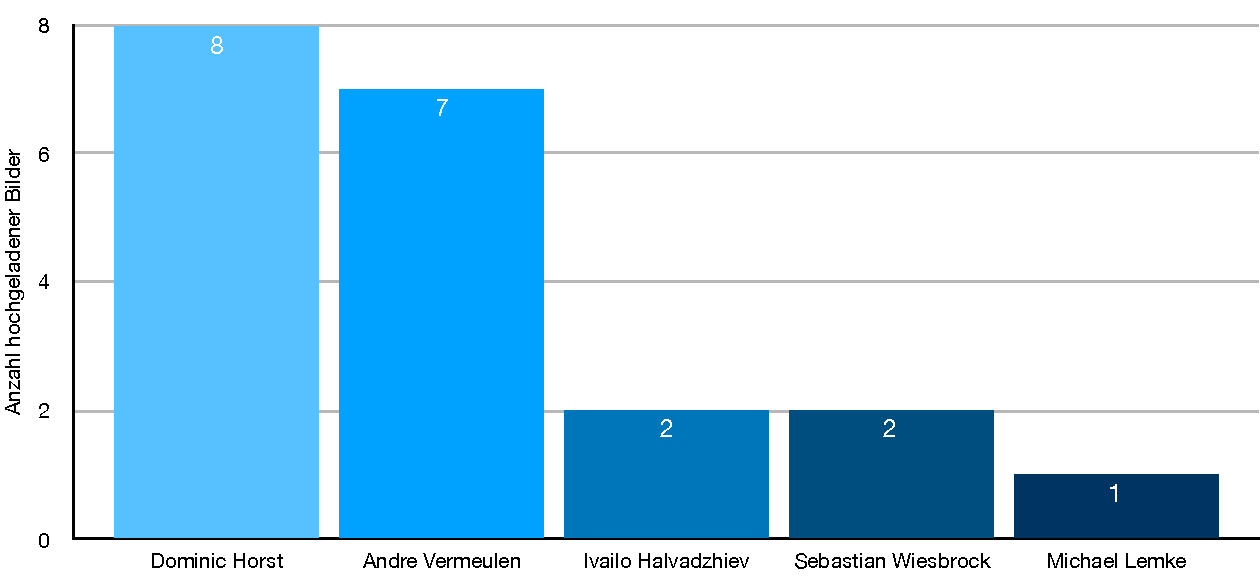
\includegraphics[keepaspectratio, width=\textwidth]{data/usage_pb}
  \caption{Anzahl hochgeladener Bilder am Standort Paderborn im Zeitraum 25. Januar bis 27. Februar 2018}
  \label{fig:usagepb}
\end{figure}

\begin{figure}[h]
  \centering
  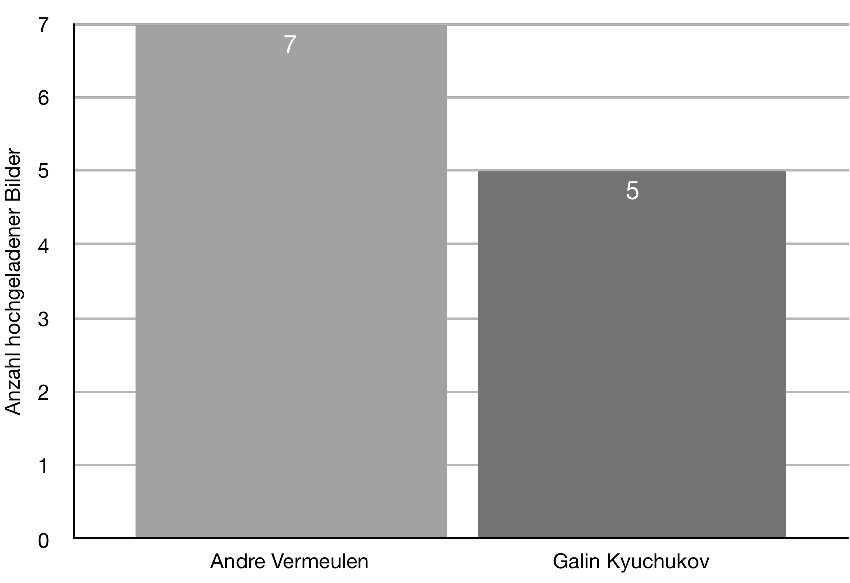
\includegraphics[keepaspectratio, width=\textwidth]{data/usage_bg}
  \caption{Anzahl hochgeladener Bilder am Standort Stara Zagora im Zeitraum 31. Januar bis 2. März 2018}
  \label{fig:usagebg}
\end{figure}
